% !TeX root = ../thesis.tex

\chapter{绪论}

作为计算机科学中的重要组成,概率算法在
排序与搜索、素数分解、多项式求根、字符串的模式匹配等方面
都有很好的应用。
概率的思想同样可以应用于并发系统的研究,
其中有代表性的工作有对CCS的概率性扩展\cite{9,10},
概率CSP\cite{11} 和概率ACP\cite{12}等。
近期,Fu提出了一个模型无关的通用方法,
可以用于将并发进程模型扩展为概率并发进程模型。
由于其模型无关性,
我们可以使用这一方法对其他并发进程模型进行概率化扩展。

\section{并发进程模型}
  20世纪70年代初期,为了保证操作系统中多个并行执行程序的正确性,
  并发程序理论由此产生。随着并行和分布式计算机系统的发展,
  并发程序理论程序理论的一个重要分支。
  并发程序理论的研究内容包括:
  如何刻画并行进程的行为,
  在什么情况下他们可以互相模拟,
  研究各种通信和同步机制,
  死锁、可观察性、发散性等并发现象。
  并发程序理论的研究加深了人们对并发系统的认识,
  其主要的研究成果已经在Ada,Java等程序语言中得到广泛应用。[cite1]

   20世纪80年代,英国学者Milner提出了通信系统演算(A Calculus of Communicating System,简称\textbf{CCS})\cite{2},
   同时期Hoare提出了CSP\cite{3},
   Bergstra和Klop等提出了ACP\cite{4},Hennessy提出ATP\cite{5}等使用代数方法研究通信并发系统,统称为进程代数理论。

   Milner的通信系统演算(以下称为CCS)可以表达操作带来的状态迁移,进程的并行执行,多种操作的选择和通道的隐藏。
   这一并发进程模型可以用标记变迁系统(Labled Transition System)表示:

   CCS的语法如下:
   $$S,T:=X\mid \sum_{i\in I}\alpha_i.T_i\mid S\mid T \mid (a)T \mid \mu X.T$$

   其中$S,T$为CCS的代理(agent),$X$为代理变元(agent variables)。索引集合$I$是有限自然数集。
   $Chan$为名字(name)的集合,其中的元素以小写字母表示,
   集合$\overline{Chan}=\{\overline{a}\mid a\in Chan\}$,
   动作集合$Act=Chan\cup \overline{Chan}\cup \{\tau\} $,
   其中的元素用小写希腊字母表示,$\alpha_i\in Act$,$\tau$表示一切内部动作。
   $\sum_{i\in I}\alpha_i.T$为非确定性选择项,若$I=\emptyset$,我们可以将这一项写作$0$。
   $S\mid T$表示$S,T$可以并发执行。$(a)T$为限制(Restriction)或本地化(Localization)操作子,对外隐藏$T$中的$a$通道,
   也可以写为$T\backslash \{a\}$或$T\backslash a$。$\mu X$表示递归(Recursion)操作。
   若一个CCS代理$P$中不含自由变元,称$P$为进程(process)。

   CCS的迁移语义如图~\ref{fig_ccs},表示状态之间的变迁规则,其中$\lambda \in Act$。

   \begin{figure}[!htbp]
    \small
    \centering
    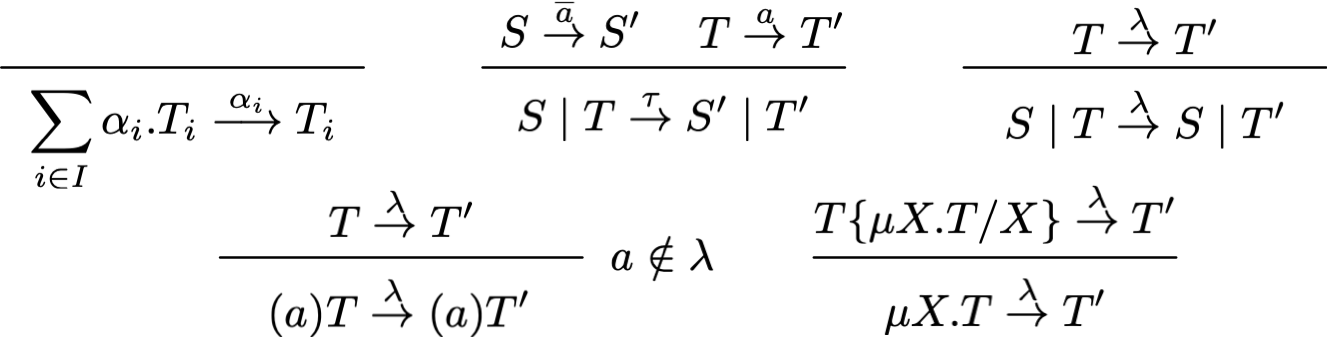
\includegraphics[width=11cm]{../figure/ccs.png}
    \caption[]{CCS迁移语义}
     \label{fig_ccs}
 \end{figure}

   CCS及其扩展模型可以用于并发系统的建模。
   提出CCS时,Milner在\cite{2}中对有界缓冲区,存在并行工作的工人的工厂,支持并行计算的编程语言进行了建模。
   基于CCS的建模还有Guo等的欧洲列车控制系统\cite{16},
   Issad等的铁路系统\cite{17},
   Cleaveland等的图坐标系语言\cite{18}等。
   CCS也可以用来评估系统特性,如判断是否出现死锁。[wiki有一个引用]
   \section{随机进程模型}

   Fu提供了一个模型无关的方法——An Uniform Approach to Random Process Model(后文称为Uniform Approach),
   进程模型扩展为随机进程模型。
   Uniform Approach区分了非确定行为和概率性的行为,
   在CCS的基础上建立了Randomized CCS(后文称为RCCS)的语法和等价关系。

   RCCS在CCS的基础上增加了概率选择操作子$\bigoplus_{i\in I}p_i\tau.T_i$,
   其中$0<p_i<1 \wedge \sum_{i\in I}p_i = 1$。
   例如,$S=\frac{1}{3}\tau.T_1+\frac{2}{3}\tau.T_2$意味着$S$经过内部动作到达$T_1$的概率为$\frac{1}{3}$,
   到达$T_2$的概率为$\frac{2}{3}$。

   对应随机选择操作子的迁移语义为:
   \begin{figure}[!htbp]
    \small
    \centering
    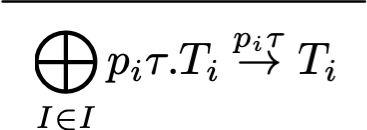
\includegraphics[width=3cm]{../figure/rccs.png}
     \label{fig_rccs}
 \end{figure}

   由于Uniform Approach具有模型无关性,我们可以用它来扩展其他的进程模型,
   进而使非概率模型概率化。概率化后,模型将会拥有更可计算、可模拟的性质。
   进而可以更好的对现实问题进行仿真和分析。

\section{研究目的}
本文希望使用Uniform Approach的通用方法,
概率化扩展经典并发模型——并发传值进程模型,得到随机传值进程模型。
我们可以通过对传值进程模型的扩展,
一方面进一步佐证Uniform Approach的模型无关性;
一方面随机传值进程模型可以应用于具有传值特点的并发系统的建模和分析,
如通信过程、安全协议、生物系统等。
我们希望随机传值进程模型的语法、迁移语义
可以用于为具有传值特点现实问题建模通信、同步等机制,
为这类问题的模型设计与软件开发提供方法,
并应用随机传值进程模型的互模拟关系、等价关系等性质
分析模型的死锁、活性、可观察、发散等并发特性。

\section{论文结构}
本文分为三个章节。第一章为绪论,引入了通信并发系统的概念,
介绍了通信并发演算CCS,引入了一种对进程模型进行概率化扩展的通用方法Uniform Approach。
第二章我们使用Uniform Approach中的方法对传值进程模型进行概率化扩展得到随机传值进程模型。
第三章我们使用随机传值进程模型对基于云计算协议Gossip-Style Membership协议的通信过程建模。
第四章为结论以及本文待改进的工作。
